% 74-20(74쪽) — $y=a\cos(bx+c)$ 의 그래프(원문 「오른쪽 그림」). 스캔 화질이 낮아 TikZ 로 다시 그림.
% 라벨은 원문 것만: $3$, $-3$, $\pt{O}$, $-\dfrac{5}{12}\pi$, $\dfrac{\pi}{12}$, $\dfrac{7}{12}\pi$, 그래프 이름.
% 원문에 없는 눈금·값은 적지 않는다. 가로축 단위는 $\pi$ 배(라벨 자리만 원문과 맞춘다).
\begin{tikzpicture}[line width=0.6pt, x=2.56cm, y=0.45cm, >=stealth]
  \draw[densely dashed, line width=0.35pt] (-0.82,3) -- (1.38,3);
  \draw[densely dashed, line width=0.35pt] (-0.82,-3) -- (1.38,-3);
  \draw[->, line width=0.7pt] (-0.86,0) -- (1.45,0) node[below=1pt, font=\small] {$x$};
  \draw[->, line width=0.7pt] (0,-4.6) -- (0,4.8) node[left=1pt, font=\small] {$y$};
  \draw[domain=-0.80:1.30, samples=200, smooth] plot (\x, {3*cos(360*\x+60)});
  \node[anchor=east, font=\small, fill=white, inner sep=1pt] at (-0.02,3) {$3$};
  \node[anchor=east, font=\small, fill=white, inner sep=1pt] at (-0.02,-3.5) {$-3$};
  \node[anchor=north east, font=\small] at (-0.01,-0.1) {$\pt{O}$};
  \node[anchor=east, font=\small] at (-0.26,1.2) {$-\dfrac{5}{12}\pi$};
  \node[anchor=south, font=\small] at (0.19,0.5) {$\dfrac{\pi}{12}$};
  \node[anchor=north, font=\small] at (0.76,-0.4) {$\dfrac{7}{12}\pi$};
  \node[anchor=west, font=\small] at (0.04,3.6) {$y=a\cos(bx+c)$};
\end{tikzpicture}
